\chapter{Methodology}

\vspace{-1cm}

This chapter shows the process of designing, testing and troubleshooting tools and equipment, construction and wiring procedure.

Now that the design is in place, the purchase of material will follow, then the construction of the device and lastly the performance,
functionality, and reliability will be tested.

\section{System Design}
\begin{figure}[ht]
  \centering \begin{tikzpicture}
    \node[anchor=north west] (battery) at (0, -0.3) {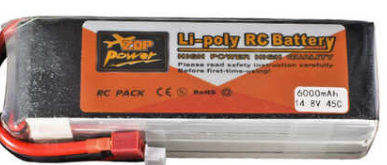
\includegraphics[width=3cm]{assets/battery.png}};
    \node[anchor=north west] (converter) at (5, 0) {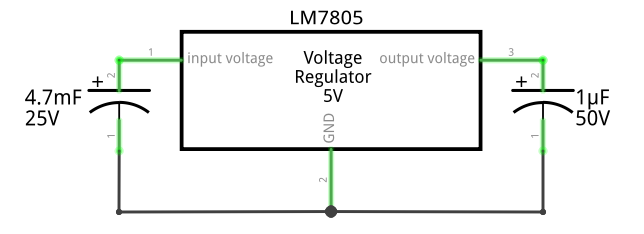
\includegraphics[width=5cm]{assets/converter.png}};
    \node[anchor=north west] (esp32) at (6, -3.5) {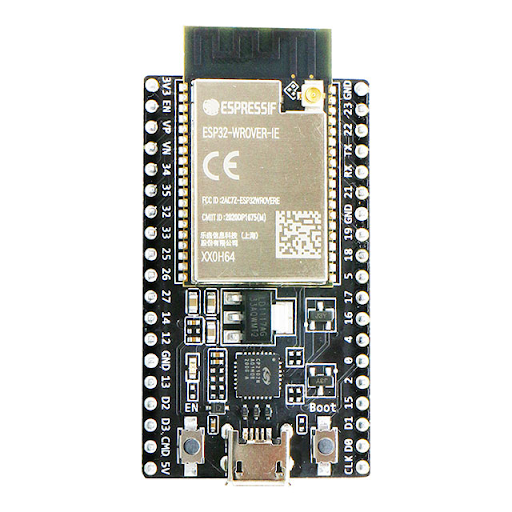
\includegraphics[width=3cm]{assets/esp-32.png}};
    \node[anchor=north west] (magnetometer) at (12, -0.5) {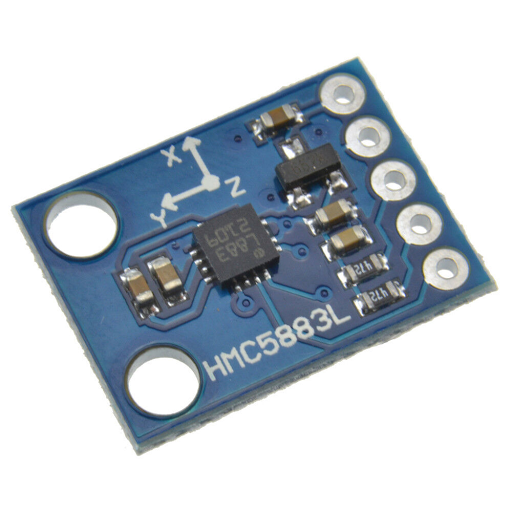
\includegraphics[width=3cm]{assets/magnetometer.png}};
    \node[anchor=north west] (gps) at (12, -6) {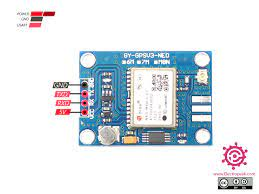
\includegraphics[width=3cm]{assets/gps_module.png}};
    \node[anchor=north west] (esc) at (0, -3.5) {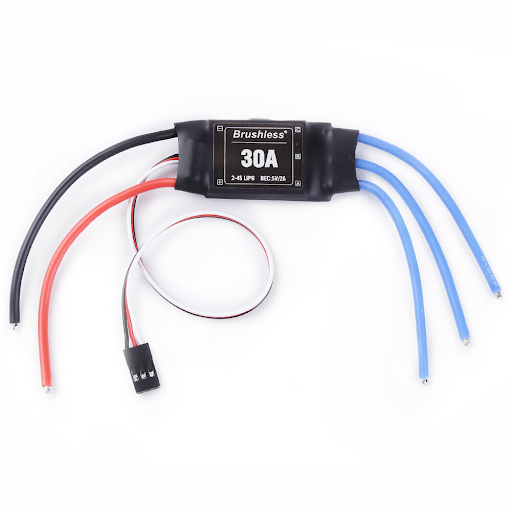
\includegraphics[width=3cm]{assets/esc.png}};
    \node[anchor=north west] (motor) at (3, -8) {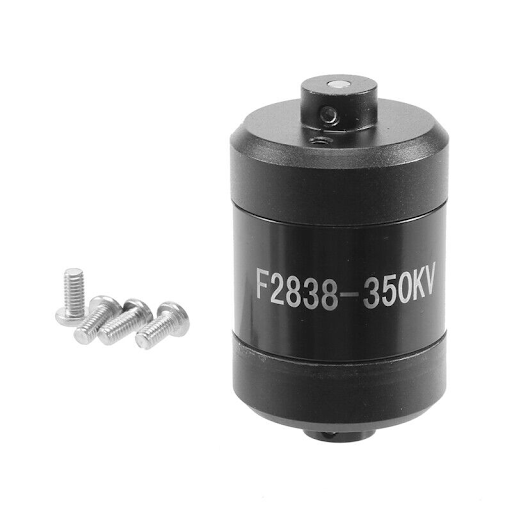
\includegraphics[width=3cm]{assets/motor.png}};
    \node[anchor=north west] (propeller) at (9, -8.2) {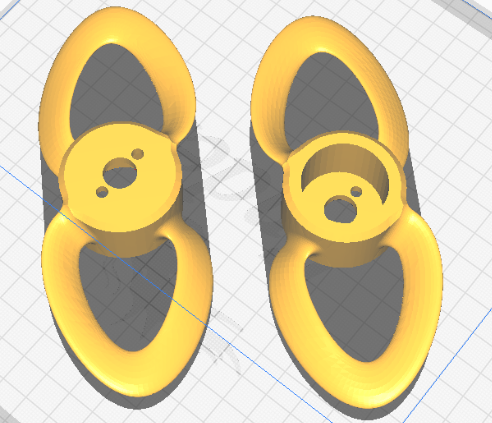
\includegraphics[width=3cm]{assets/propellers.png}};

    \draw[ ->, line width = 1mm, black!70] (battery) to (converter);
    \draw[ ->, line width = 1mm, black!70] (battery) to (esc);
    \draw[ ->, line width = 1mm, black!70] (esp32) to (esc);
    \draw[ <->, line width = 1mm, black!70] (esc) |- (motor);
    \draw[ ->, line width = 1mm, black!70] (motor) to (propeller);
    \draw[ ->, line width = 1mm, black!70] (converter) to (esp32);
    \draw[ <->, line width = 1mm, black!70] (esp32.east) + (0, 0.3) -| (magnetometer.south);
    \draw[ <->, line width = 1mm, black!70] (esp32.east) + (0, -0.2) -| (gps.north);

    % \path[ ->, line width = 1mm, black!70] (esp32.east) + (0, 1) edge [bend left] (magnetometer);
    % \path[ <-, line width = 1mm, black!70] (esp32.east) + (0, 0.5) edge [bend right] (magnetometer.west);
    % \path[ ->, line width = 1mm, black!70] (esp32.east) + (0, -0.5) edge [bend right] (gps);
    % \path[ <-, line width = 1mm, black!70] (esp32.east) + (0, 0) edge [bend left] (gps.west);


  \end{tikzpicture}
  \caption{System Design}
  \label{fig:SystemDesign}
\end{figure}

\pagebreak

% \section{Flowchart}
% \begin{figure}[ht]
% \centering \begin{tikzpicture}
%   [
%   RECT/.style={rectangle, rounded corners, draw=black!60, fill=white!0, very thick, minimum width = 20mm, minimum height = 10mm, align = center},
%   ROUNDEDRECT/.style={rounded rectangle, draw=black!60, fill=white!0, very thick, minimum width = 20mm, minimum height = 10mm},
%   DIAMOND/.style={diamond, draw=black!60, fill=white!0, very thick, minimum width = 10mm, minimum height = 10mm, align = center, aspect = 2, },
%   ]

%   \node[ROUNDEDRECT] (start) {Start};
%   \node[RECT] (switchOn) [below = of start] {Switch on};
%   \node[RECT] (esp32Boot) [right = of switchOn] {ESP-32 boots};
%   \node[RECT] (waitForUserInput) [right = of esp32Boot] {Waiting for user \\ input coordinates};
%   \node[RECT] (coordinatesSupplied) [below = of waitForUserInput] {Coordinates Supplied};
%   \node[RECT] (detectsLocationData) [left = of coordinatesSupplied] {GPS \& magnetometer \\ detects location data};
%   \node[RECT] (droneMoves) [left = of detectsLocationData] {Drone moves to \\ supplied coordinates};
%   \node[RECT] (confirmLoc) [below = of droneMoves] {GPS \& magnetometer \\ confirms location data};
%   \node[] (dummyNode) [below = of detectsLocationData] {};
%   \node[DIAMOND] (doesLocMatch) [below = of dummyNode] {Does drone location match \\ with supplied coordinates?};
%   \node[RECT] (terminate) [below = of doesLocMatch] {Drone terminated};
%   \node[ROUNDEDRECT] (end) [right = of terminate] {End};

%   \draw[ ->, line width = 1mm, black!70] (start.south) to node[] {} (switchOn.north);
%   \draw[ ->, line width = 1mm, black!70] (switchOn.east) to node[] {} (esp32Boot.west);
%   \draw[ ->, line width = 1mm, black!70] (esp32Boot.east) to node[] {} (waitForUserInput.west);
%   \draw[ ->, line width = 1mm, black!70] (waitForUserInput.south) to node[] {} (coordinatesSupplied.north);
%   \draw[ ->, line width = 1mm, black!70] (coordinatesSupplied.west) to node[] {} (detectsLocationData.east);
%   \draw[ ->, line width = 1mm, black!70] (detectsLocationData.west) to node[] {} (droneMoves.east);
%   \draw[ ->, line width = 1mm, black!70] (droneMoves.south) to node[] {} (confirmLoc.north);
%   \draw[ ->, line width = 1mm, black!70] (confirmLoc.south) to node[] {} (doesLocMatch.west);
%   \draw[ ->, line width = 1mm, black!70] (doesLocMatch.north) to node[left] {NO} (detectsLocationData.south);
%   \draw[ ->, line width = 1mm, black!70] (doesLocMatch.south) to node[left] {YES} (terminate.north);
%   \draw[ ->, line width = 1mm, black!70] (terminate.east) to node[] {} (end.west);
% \end{tikzpicture}
% \caption{Flowchart}
% \label{fig:Flowchart}
% \end{figure}

\section{Flowchart}
\begin{figure}[ht]
  \centering \begin{tikzpicture}
    [
      RECT/.style={rectangle, rounded corners, draw=black!60, fill=white!0, very thick, minimum width = 20mm, minimum height = 10mm, align = center},
      ROUNDEDRECT/.style={rounded rectangle, draw=black!60, fill=white!0, very thick, minimum width = 20mm, minimum height = 10mm},
      DIAMOND/.style={diamond, draw=black!60, fill=white!0, very thick, minimum width = 10mm, minimum height = 10mm, align = center, aspect = 3, },
    ]

    \node[ROUNDEDRECT] (start) {Start};
    \node[RECT] (switchOn) [right = of start] {Switch on};
    \node[RECT] (waitForUserInput) [below right = of switchOn] {Waiting for \\ user to provide \\ target coordinates};
    \node[RECT] (waitingForSensor) [below left = of switchOn] {Waiting for GPS and \\ magnetometer modules to \\ process  location and heading};
    \node[DIAMOND] (isUserInputValid) [below = of waitForUserInput] {Is user input \\ valid?};
    \node[DIAMOND] (isSensorDataValid) [below = of waitingForSensor] {Is sensor data \\ valid?};
    \node[RECT] (compute) [below = 5.5cm of switchOn] {Compute distance and \\ bearing to target};
    \node[RECT] (move) [below = of compute] {Drone turns and \\ moves to target};
    \node[DIAMOND] (distance) [below = of move] {Is the distance between \\ the drone and the target within the \\ uncertainty threshold?};
    \node[RECT] (terminate) [below = of distance] {Drone terminated};
    \node[ROUNDEDRECT] (end) [right = of terminate] {End};

    \draw[ ->, line width = 1mm, black!70] (start) to (switchOn);
    \draw[ ->, line width = 1mm, black!70] (switchOn.south) + (3mm, 0) |- (waitForUserInput.west);
    \draw[ ->, line width = 1mm, black!70] (switchOn.south) + (-3mm, 0) |- (waitingForSensor.east);
    \draw[ ->, line width = 1mm, black!70] (waitForUserInput) to (isUserInputValid);
    \draw[ ->, line width = 1mm, black!70] (waitingForSensor) to (isSensorDataValid);
    \draw[ ->, line width = 1mm, black!70] (isSensorDataValid.south)  |- node[below] {Yes} (compute.west);
    \draw[ ->, line width = 1mm, black!70] (isUserInputValid.south) |- node[below] {Yes} (compute.east);
    \draw[ ->, line width = 1mm, black!70] (compute) to (move);
    \draw[ ->, line width = 1mm, black!70] (move) to (distance);
    \draw[ ->, line width = 1mm, black!70] (distance) to node[left] {Yes} (terminate);
    \draw[ ->, line width = 1mm, black!70] (terminate) to (end);
    \draw[ ->, line width = 1mm, black!70] (isSensorDataValid) + (-3, 0) node[below] {No} |- (waitingForSensor.west);
    \draw[ -, line width = 1mm, black!70] (waitingForSensor) + (-3, 0) |- (isSensorDataValid.west);
    \draw[ ->, line width = 1mm, black!70] (isUserInputValid) + (3, 0) node[below] {No} |- (waitForUserInput.east);
    \draw[ -, line width = 1mm, black!70] (waitForUserInput) + (3, 0) |- (isUserInputValid.east);
    \draw[ ->, line width = 1mm, black!70] (distance) + (-6, 0) node[below] {No} |- (move.west);
    \draw[ -, line width = 1mm, black!70] (move) + (-6,0) |- (distance.west);

  \end{tikzpicture}
  \caption{Flowchart}
  \label{fig:Flowchart}
\end{figure}

\section{Navigation algorithm}
\begin{enumerate}
  \item  Get target location \tLoc from the user

        \tLoc is acquired from the user by specifying its geo-coordinates in the \emph{Latitude-Longitude} format. Latitude values denote the angular distance relative
        to the equator, with positive values indicating locations north of the equator and negative values indicating locations south of the equator. Similarly, Longitude values
        represent the angular distance east or west of the Prime Meridian, with positive values corresponding to western locations and negative values signifying eastern locations.
        \emph{Both Latitude and Longitude should be specified as decimal degrees.}

  \item  Get current location \cLoc and current heading \heading from GPS and magnetometer modules

        \cLoc is acquired from the Global Positioning System (GPS) module. The module transmits NMEA sentences (refer to Section X.X todo for a detailed
        explanation) to the ESP32 microcontroller.  Of these sentences, the GPGLL sentence is specifically processed to extract the latitude, north/south (N/S) indicator, longitude,
        east/west (E/W) indicator, and validity status.  The latitude and longitude values are converted from the degrees-minutes-decimal minutes format (dddmm.mmmm)
        to decimal degrees for further calculations.  Subsequently, the N/S and E/W indicators are used to determine the correct sign (positive or negative) for the extracted
        latitude and longitude values.

        In contrast, \heading is calculated based on the \emph X and \emph Y values obtained from the magnetometer module.
        This value represents the device's orientation relative to magnetic north. The calculation of \heading requires the declination angle \decAngle which is itself derived from the
        longitude component of the current location, \cLoc. The declination correction accounts for the difference between magnetic north and true geographic north.  This correction is
        applied to the magnetic heading which is an azimuth value between 0 and 359 degrees, to obtain a value that represents the device's orientation relative to
        true north.
        $$ \theta_c = \atantwo(y, x) + \frac{180}{\pi} + (\underbrace{0.015}_{\mathclap {\text{\hspace{+3.5cm} constant used to approximate angle of declination}}} * X_c^\lambda) + 1 $$

        A specific function is then used to ensure the resulting value remains within the 0 to 359 degree range and avoids overflow errors.


  \item Get the difference between between the longitude \longDiff and latitude \latDiff components of \cLoc and \tLoc
        \begin{align*}
          \lambda & = X_c^\lambda - X_t^\lambda \\
          \phi    & = X_c^\phi - X_t^\phi
        \end{align*}

  \item Get distance \distance between \cLoc and \tLoc

        Due to the Earth's oblateness, getting the distance between two geographic coordinates presents complexities. The conversion factor required for accurate
        transformation varies depending on the specific location on the Earth's surface. To address this, we will leverage an approximate formula used in the source
        code of CSGNetwork.com's length of a degree of latitude and longitude calculator\cite{sourcecode}. This formula was further explored in an answer in a forum post in the
        Geographic Information Systems Stack Exchange website\cite{forum} indicating that it was derived from the WGS84 ellipsoidal Earth model.

        $$ \phi_m = \frac{X_c^\phi + X_t^\phi}{2} $$
        \begin{align*}
          \phi_d = \text{ meters per degree in } \phi       & = 111132.92 \; - \; 559.82\cos2{\phi_m}       \\ & \quad +  \; 1.175cos4\phi_m \; - \; 0.0023\cos6\phi_m \\ \\
          \lambda_d = \text{ meters per degree in } \lambda & = 111412.84\cos\phi_m \; - \; 93.5\cos3\phi_m \\ & \quad + \; 0.118\cos5\phi_m
        \end{align*}

        To find the distance in meters, we will apply the Pythagorean Theorem.

        $$ \Delta = \sqrt{{(\phi_d)}^2 + {(\lambda_d)}^2} $$

  \item Get target bearing \bearing from \cLoc to \tLoc

        Assuming that the \cLoc and \tLoc is in a two-dimensional Cartesian plane centered at \cLoc, we determine \bearing using the \emph{atan} function and
        quadrant-specific adjustments. The \emph{arctangent}, expressed as $\arctan(\frac{\lambda}{\phi})$ calculates the fundamental inclination angle. To account for the
        varying quadrants and to ensure an accurate directional representation from the origin, corrective terms of 180\degrees or 360\degrees are incorporated based
        on the signs of \longDiff and \latDiff. This simple approach offers a robust and computationally efficient method for calculating azimuths within the assumed two-dimensional
        spatial framework.

        $$ \theta_t = \begin{cases}
            \arctan(\frac{\lambda}{\phi})       & \text{if } \lambda > 0 \text{ and } \phi > 0 \rightarrow \text{quadrant 1} \\
            \arctan(\frac{\lambda}{\phi}) + 180 & \text{if } \lambda > 0 \text{ and } \phi < 0 \rightarrow \text{quadrant 2} \\
            \arctan(\frac{\lambda}{\phi}) + 180 & \text{if } \lambda < 0 \text{ and } \phi < 0 \rightarrow \text{quadrant 3} \\
            \arctan(\frac{\lambda}{\phi}) + 360 & \text{if } \lambda < 0 \text{ and } \phi > 0 \rightarrow \text{quadrant 4} \\
          \end{cases} $$

  \item Calculate relative bearing \rBearing between \bearing and \heading

        The raw relative bearing $\boldsymbol{\delta}$ is subsequently calculated by subtracting the measured heading \heading from the target bearing \bearing.

        $$ \delta = \theta_c - \theta_t $$

        To constrain \rBearing within the range of -180\degrees \space to 180\degrees, a correction step is implemented to the raw relative bearing. If the absolute value of $\delta$ exceeds
        180\degrees, the absolute value $\delta$ is subtracted from 360\degrees. This ensures that \rBearing remains as close to zero as possible.
        A minimal relative bearing value translates to the smallest required turning angle.

        $$ \theta = \begin{cases}
            \delta         & \text{if } |\delta| \leq 180 \\
            360 - |\delta| & \text{if } |\delta| > 180
          \end{cases} $$

  \item Differential thrust for yaw control
  
        To achieve yaw (turn) maneuvers, the relative bearing, \rBearing, dictates the power distribution between the designated motors. Positive \rBearing signifies a turn
        towards the port side (left), while negative \rBearing corresponds to a starboard (right) turn.

        To generate yaw torque, one motor experiences a reduction in thrust while the opposing motor stays at the maximum thrust. For a port turn, the port motor's thrust is reduced
        and the starboard motor's thrust stays at the maximum. Conversely, a starboard turn necessitates the opposite configuration.

        To minimize the duration of reduced thrust on a single motor and reduce transient effects, a damping value function is implemented. When the relative bearing is within a predefined
        tolerance zone of 5\degrees$\pm$, both motors operate at full capacity, effectively maintaining straight travel.

        For relative bearings exceeding the tolerance thresholds, the thrust of the appropriate motor is reduced linearly. In a scenario requiring a full port turn, the port motor's thrust 
        would be linearly reduced to zero while the starboard motor maintains maximum thrust. Conversely, a full starboard turn would involve linearly scaling the starboard motor's thrust to 
        zero while maintaining maximum thrust on the port motor.

        When the drone's distance to the target, designated by \distance, is within the \emph{uncertainty threshold}, both of the motors would provide no thrust. If \distance has increased to 
        above the \emph{uncertainty threshold} due to drift, then the algorithm will loop back up again and try to correct the drift.
\end{enumerate}

When the distance to the target, \distance, falls within the \emph{uncertainty threshold}, both motors are commanded to produce zero thrust as the target is sufficiently close. However,
if the distance exceeds the \emph{uncertainty threshold} due to factors such as environment disturbance or drift, the control algorithm iterates back to the beginning and initiates corrective
actions to re-establish accurate positioning relative to the target.

\section{Construction Procedure}

\section{Testing and Evaluation}

\section{Sources of Data}

\section{Project Components and Materials}

\section{Instruments}
